\documentclass[12pt,a4paper]{article}
\usepackage{rmpackages}																% usual packages
\usepackage{rmtemplate}																% graphic charter
\usepackage{rmexocptce}																% for DS with cptce eval

%\cfoot{} 													% if no page number is needed
%\renewcommand\arraystretch{1.5}		% stretch table line height

\begin{document}
\begin{header}
Mesurer une molécule -- Fiche prof
\end{header}

\section{L'activité}

\subsection{Déroulement de la séance}

\paragraph{Accueil :}
\begin{itemize}
\item[•] Accueil des élèves, désinfection des mains, placement libre par binôme
\item[•]\og Bonjour à tous, asseyez-vous. \fg{}
\item[•] Appel.
\end{itemize}

\paragraph{Présentation de la séance :}
\begin{itemize}
\item[•] Contextualisation : 

\og Rappelez vous le titre du chapitre 3, du macroscopique au microscopique : on part d'une description de la matière à notre échelle pour aller en venir à l'étude des particules qui composent la matière.
Avec l'activité d'aujourd'hui c'est exactement le chemin que l'on va suivre : on va interpréter une expérience macroscopique, à notre échelle, pour déterminer la taille d'une molécule d'huile.
On va essayer répondre à la question :

\textsc{Quelle est la taille d'une molécule d'huile ?}\fg{} 

\item[•] \og Tout le mode écoute, je vous donne les consignes générales.\fg{}

\item[•] Consignes :
\begin{itemize}
\item Objectif : répondre à la question \og quelle est la taille d'une molécule d'huile ? \fg{}
\item Pour répondre vous allez rédiger un compte-rendu : la première étape sera comme d'habitude de donner votre hypothèse \og Je pense qu'une molécule d'huile mesure ... car ... \fg{}
\item Pour la suite vous vous aiderez de l'aide écrite dans le sujet.
\item Un CR chacun, j'en ramasserai un par groupe au hasard à la fin.
\end{itemize}

\item[•] Est-ce qu'il y a des questions ?

C'est bon pour tout le monde ?

Je vous distribue le sujet et c'est parti.
\end{itemize}

\paragraph{Préparer la fiche de notation avec le nom des binômes.}

\paragraph{Première aide}
\begin{itemize}
\item[•] Coup de pouce : Commencez par déterminer le volume d'une cuillère à café.
\item[•] Aide : Quelle verrerie peut-on utiliser pour mesurer un volume ?
\item[•] Aide : Mesure le volume d'une cac d'huile avec une éprouvette.
\item[•] Aide : Une cac fait 2 mL.
\end{itemize}

\paragraph{Deuxième aide}
\begin{itemize}
\item[•] Coup de pouce : Dessinez la tache d'huile en 3D.
\item[•] Aide : À quoi correspondent les différentes grandeurs dans la formule, les quelles sont connues ?
\item[•] Aide : Mesure l'aire sur le schéma
\item[•] Aide : L'aire de la flaque est \unit{2000}{m\squared}
\end{itemize}

\paragraph{Troisième aide}
\begin{itemize}
\item[•] Coup de pouce : Pourquoi la tache arrête-t-elle de s'étendre ?
\item[•] Aide : Ça vous semble normal de trouver un chiffre aussi petit ?
\item[•] Aide : Le professeur verse des haricots sur la table
\item[•] Aide : L'huile forme une couche haute comme une seule molécule
\end{itemize}

\paragraph{Nettoyage}

\paragraph{Ramasser les compte-rendus}
 
\paragraph{Fin de la séance}

\subsection{Matériel}

Le matériel est à disposition des élèves mais pas directement sur leur paillasse :
\begin{itemize}
\item[•] bécher \unit{100}{mL} ;
\item[•] éprouvette graduée \unit{10}{mL} ;
\item[•] balance ;
\item[•] cuillère à café ;
\item[•] entonnoir ;
\item[•] eau ;
\end{itemize}

\section{Évaluation}

Lors de la séance, l'évaluation est portée sur trois compétences en particulier : \anarai{}, \rea{} et \val{}.\footnote{Puisque l'activité est un problème ouvert, d'autres compétences sont inévitablement mobilisées mais il est possible de les évaluer après la séance sur la base du compte-rendu rédigé par les élèves.
Ce n'est pas sur celles-ci que l'accent est mis pour cette activité.}
La maitrise de ces compétences est graduée selon quatre niveaux identifiables d'après l'aide apportée lors de la séance : A (bien maitrisée), B (maitrisée), C (insuffisamment maitrisée) et D (non maitrisée).
Les observables sont définies dans le tableau~\ref{tab:obs}.

\begin{table}
\center
\begin{tabular}{l|l|c}
\textbf{Compétence} & \textbf{Aptitude} / Observable & \textbf{Niveau} \\
\hline \hline
\anarai 	& \textbf{Élaborer un protocole qui répond à la question} 	& \\
				& L'élève mesure le volume de 10 cac				 						& A+ \\
				& L'élève mesure le volume d'une cac 									& A \\
				& Aide : Avec quelle verrerie peut-on mesurer un volume ?	& B \\
				& Aide : Mesure le volume d'une cac d'huile avec une éprouvette & C \\
				& Aide : Une cac fait 5 mL 															& D \\
\hline
\rea			& \textbf{Faire des observations utiles à l'activité}					& \\
				& L'élève réalise la mesure de l'aire sur le schéma				& A \\
				& Aide : Dans la formule, quelles sont les valeurs connues ? & B \\
				& Aide : Mesure l'aire sur le schéma											& C \\
				& Aide : L'aire de la flaque est \unit{2000}{m\squared}			& D \\
\hline
\val			& \textbf{Avoir un regard critique sur ses résultats}				& \\
				& L'élève fait le lien avec son hypothèse									& A \\
				& Aide : Ça vous semble normal de trouver un chiffre aussi petit ? & B \\
				& Aide : Le professeur verse des haricots sur la table			& C \\
				& Aide : L'huile forme une couche haute comme une seule molécule & D \\
\end{tabular}
\caption{Observables utilisées pour l'évaluation du niveau de maitrise des compétences travaillées lors de la séance.}
\label{tab:obs}
\end{table}

\section{Analyse a priori}

Le lien entre l'aspect réellement macroscopique de cette expérience et son interprétation microscopique est sans doute une des principales difficultés de cette activité.
(lien entre espèce chimique et entité chimique présent dans les programmes et abordé en cours)

Si un élève demande à quoi ressemble une molécule d'huile, on peut montrer une molécule d'acide oléique (Fig.~\ref{fig:oleine}).
\footnote{Le composé majoritaire de l'huile d'olive est l'oléine, ou trioléine est un ester dont l'hydrolyse forme l'acide oléique et le glycérol.}
La dimension d'un atome ayant été donnée en cours, on peut s'attendre à ce que l'élève compte les atomes qui composent la \og molécule d'huile \fg{} pour estimer sa taille.
\footnote{Les élèves ont fait une activité similaire en comptant les atomes qui composent le bonhomme du film \href{https://www.youtube.com/watch?v=oSCX78-8-q0}{A boy and his atom} pour estimer sa taille.}
Il se pourrait alors que la forme allongée de la molécule induise un questionnement sur la bonne dimension à prendre en compte.
On peut différer la réponse à cette question en attendant de voir ce que donne les résultats des mesures et calculs et en reparler à la fin du TP : \og D'après vous, comment s'orientent les molécules à la surface de l'eau ? \fg{}.

\begin{figure}
\center
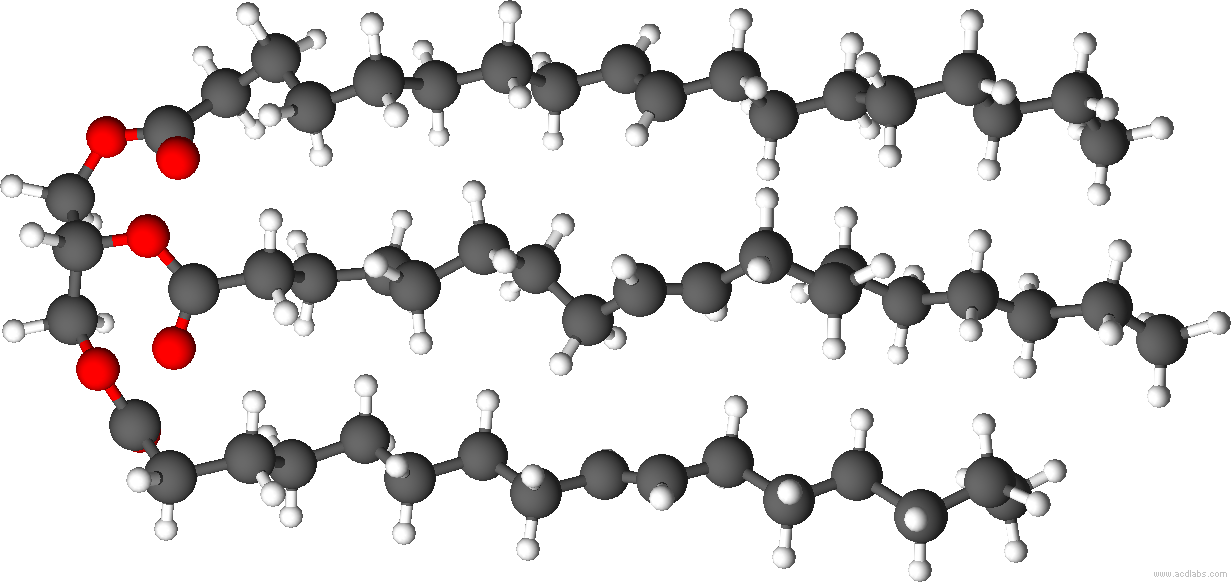
\includegraphics[scale=0.35]{images/oleine.png}
\caption{Structure d'une molécule d'oléine.}
\label{fig:oleine}
\end{figure}

On peut s'attendre à deux méthodes pour la mesure du volume de la cuillère à café : mesure \og directe \fg{} à l'aide d'une éprouvette graduée ou mesure \og indirecte \fg{} à l'aide d'une balance en passant par la masse volumique.  
Dans les deux cas, l'idée de mesurer le volume de plusieurs cuillerées sera valorisé.

On peut s'attendre aussi à ce que l'élève connaisse la valeur du volume d'une cac, ce qui relève plutôt de la compétence \app{} (évaluer quantitativement les grandeurs physiques inconnues et non précisées).
Si la valeur est bonne et que l'élève termine rapidement, on peut l'orienter sur la mesure du volume de la cuillère en l'encourageant à vérifier son hypothèse.

Le premier coup de pouce \og mesure du volume d'une cac \fg{} est individuel pour ne pas décourager différentes méthodes de résolution, comme partir sur la mesure de l'aire en premier. 

Le schéma du document 2 peut induire un biais : l'étendue de la tache d'huile est simplement repérable par l'absence de vague et pas par sa couleur.
L'épaisseur finale de l'ordre du nanomètre est beaucoup trop faible pour qu'on puisse la repérer optiquement.


\end{document}